\documentclass[tikz,border=8pt]{standalone}
% Shared look for every TikZ diagram. Load with \input{../../tools/tikz-style.tex}
\usepackage[T1]{fontenc}
\usepackage{lmodern}
\renewcommand{\sfdefault}{lmr}  % diagrams use the same serif as the text
\usetikzlibrary{arrows.meta, positioning, shapes.geometric, calc, fit, backgrounds}
\definecolor{cblue}{HTML}{4C78A8}
\definecolor{corange}{HTML}{F58518}
\definecolor{cgreen}{HTML}{54A24B}
\definecolor{cred}{HTML}{E45756}
\definecolor{cpurple}{HTML}{B279A2}
\definecolor{cgrey}{HTML}{6B6B6B}
\tikzset{
  every picture/.style={font=\sffamily, line width=1.2pt},
  box/.style={draw=#1, fill=#1!12, rounded corners=4pt, align=center, inner sep=7pt, minimum height=1.1cm},
  box/.default=cgrey,
  arrow/.style={-{Stealth[length=3mm]}, draw=cgrey, line width=1.4pt},
  title/.style={font=\sffamily\bfseries\Large},
  note/.style={font=\sffamily\small, text=cgrey, align=center},
}
\AtBeginDocument{\hyphenpenalty=10000 \exhyphenpenalty=10000}

\begin{document}
% Section 5: an embedding layer is a lookup table. "bank" picks the same row in both phrases, so it gets the same
% vector whatever its neighbours.
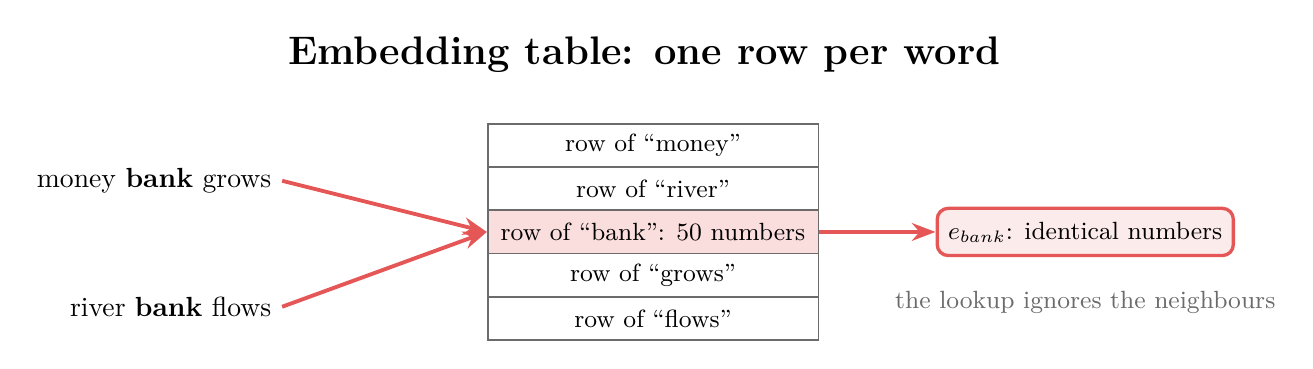
\begin{tikzpicture}[r/.style={draw=cgrey, minimum width=4.2cm, minimum height=0.55cm, font=\sffamily\small, anchor=west, line width=0.6pt},
                    w/.style={font=\sffamily}]
  \node[title] at (5.0, 2.6) {Embedding table: one row per word};
  \foreach \v [count=\i] in {money, river, bank, grows, flows} {
    \ifnum\i=3 \node[r, fill=cred!20] (row\i) at (3.0, 2.0 - 0.55*\i) {row of ``\v'': 50 numbers};
    \else \node[r] (row\i) at (3.0, 2.0 - 0.55*\i) {row of ``\v''};\fi
  }
  \node[w, anchor=east] (p1) at (0.4, 1.0) {money \textbf{bank} grows};
  \node[w, anchor=east] (p2) at (0.4, -0.6) {river \textbf{bank} flows};
  \draw[arrow, draw=cred] (p1.east) -- (row3.west);
  \draw[arrow, draw=cred] (p2.east) -- (row3.west);
  \node[box=cred, minimum height=0.6cm, inner sep=4pt, font=\sffamily\small] (out) at (10.6, 0.35) {$e_{\text{bank}}$: identical numbers};
  \draw[arrow, draw=cred] (row3.east) -- (out.west);
  \node[note] at (10.6, -0.55) {the lookup ignores the neighbours};
\end{tikzpicture}
\end{document}
